\section{General simulation setup}\label{sec:simsetup}

In the past, the simulator has been used to mimic an existing snake robot prototype, namely the Mamba snake robot \cite{liljeback2014mamba}. This snake robot has 14 identical links and 13 joints connecting these links. The visualization of the model can be seen in Figure \ref{fig:gazebo_gui}. In order to make computations simpler and thus the real time factor of the simulation higher, the robot is scaled down to have 6 links and 5 joints for some of the experiments. As can be observed from the figure, the joints are not modeled as mechanical parts. They are thus not visible, but placed mid-air between two neighboring links.
Further model details can be found in Table \ref{tab:snake_model_props}. This table shows that the links of the snake robot model have three dimensional properties, meaning both width, length and height. All experiments are however still only conducted in the two dimensional ground plane.

\begin{table}[]
    \centering
    \begin{tabular}{|c|c|c|}
        \hline
        & Value & Unit\\
        \hline
        Link mass & $1$ & $[kg]$ \\
        Link length & $0.2$ & $[m]$ \\
        Link height & $0.1$ & $[m]$ \\
        Link width & $0.1$ & $[m]$ \\
        Joint offset & $0.3$ & $[m]$\\
        \hline
    \end{tabular}
    \caption{Simulated snake robot model properties}
    \label{tab:snake_model_props}
\end{table}

When it comes to the configuration of the obstacles, it is based on the \textit{obstacle triplet model} \cite{sanfilippo2018snakesim}. The motivation behind this is explained in section \ref{sec:obst_triplet_model}. The three obstacles are modeled as identical immovable cylinders in the simulator. Still, any contact with the snake robot is a frictionless point contact. Further details about the obstacle model can be found in Table \ref{tab:obst_model_props}.

\begin{table}[]
    \centering
    \begin{tabular}{|c|c|c|}
        \hline
        & Value & Unit\\
        \hline
        Number of obstacles & $3$ & \\
        Mass & $1$ & $[kg]$ \\
        Radius & $0.1$ & $[m]$ \\
        Height & $0.2$ & $[m]$ \\
        \hline
    \end{tabular}
    \caption{Simulated obstacle model properties}
    \label{tab:obst_model_props}
\end{table}

Not all available nodes have been employed for the experiments conducted in this project. An overview of the relevant nodes and the information flow between them is presented in Figure \ref{fig:proj_nodes}. The nodes are depicted as blue ovals and the arrows describe the messages passed between them through topics.

\begin{figure}
    \centering
    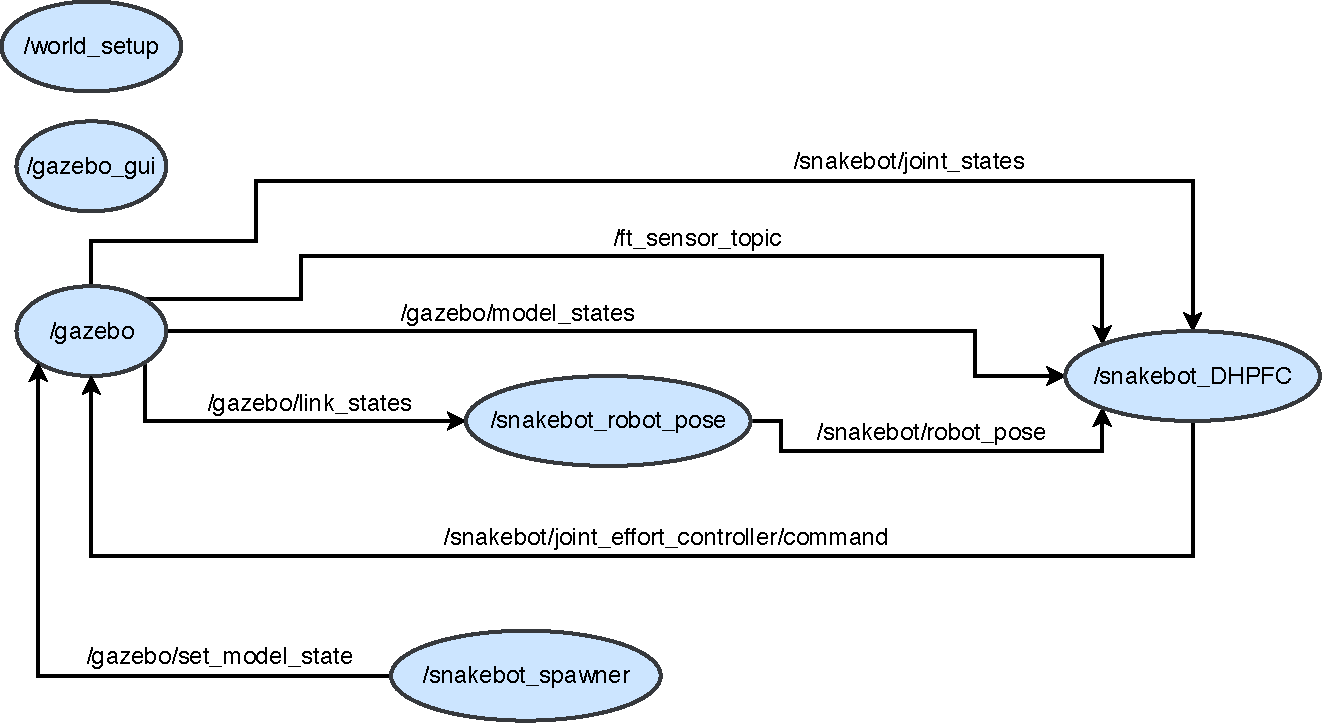
\includegraphics[width=1\textwidth]{figures/simulator/proj_nodes.pdf}
    \caption{Overview of nodes and topics used in the project experiments}
    \label{fig:proj_nodes}
\end{figure}

Furthermore, a list of the most useful topics for high level control are listed below.

\begin{itemize}
    \item \texttt{"/snakebot/pushpoints"}\\
    Information about the detected obstacle pushpoints. This includes contact normals and tangents, as well as position of contact point and information about which links are in contact with an obstacle.
    
    \item \texttt{"/snakebot/robot\char`_pose"}\\
    Global position of all snake robot links/joints??
    
    \item \texttt{"/snakebot/joint\char`_states"}\\
    Angles of all joints relative to their preceding link. This topic also provides the corresponding velocity of the joints.
    
    \item \texttt{"/snakebot/joint\char`_01\char`_effort\char`_controller/command"}\\
    Joint torque command to the specific joint actuators 
    
    \item \texttt{"/ft\char`_sensor\char`_topic\char`_01"}\\
    Wrench in specific joint measured by the force/torque sensor in Gazebo 
\end{itemize}